\part{PDEs on Bounded Domains}

\section{The Wave Equation}

\subsection{Waves on an elastic string}
Consider a small displacement $y(x,t)$ on a stretched string with fixed ends at $x = 0$ and $x = L$, that is, with boundary conditions
\begin{align} \label{eq:3.1}
	y(0,t) = y(L,t) = 0.
\end{align} 
and initial conditions
\begin{align} \label{eq:3.2}
	y(x, 0) = p(x),\ \frac{\partial y}{\partial t}(x,0) = q(x)
\end{align} 
We derive the equation of motion governing the motion of the string by balancing forces on a string segment $(x,x+\delta x)$ and take the limit as $\delta x \to 0$.
\begin{figure}[h] 
	\centering 
	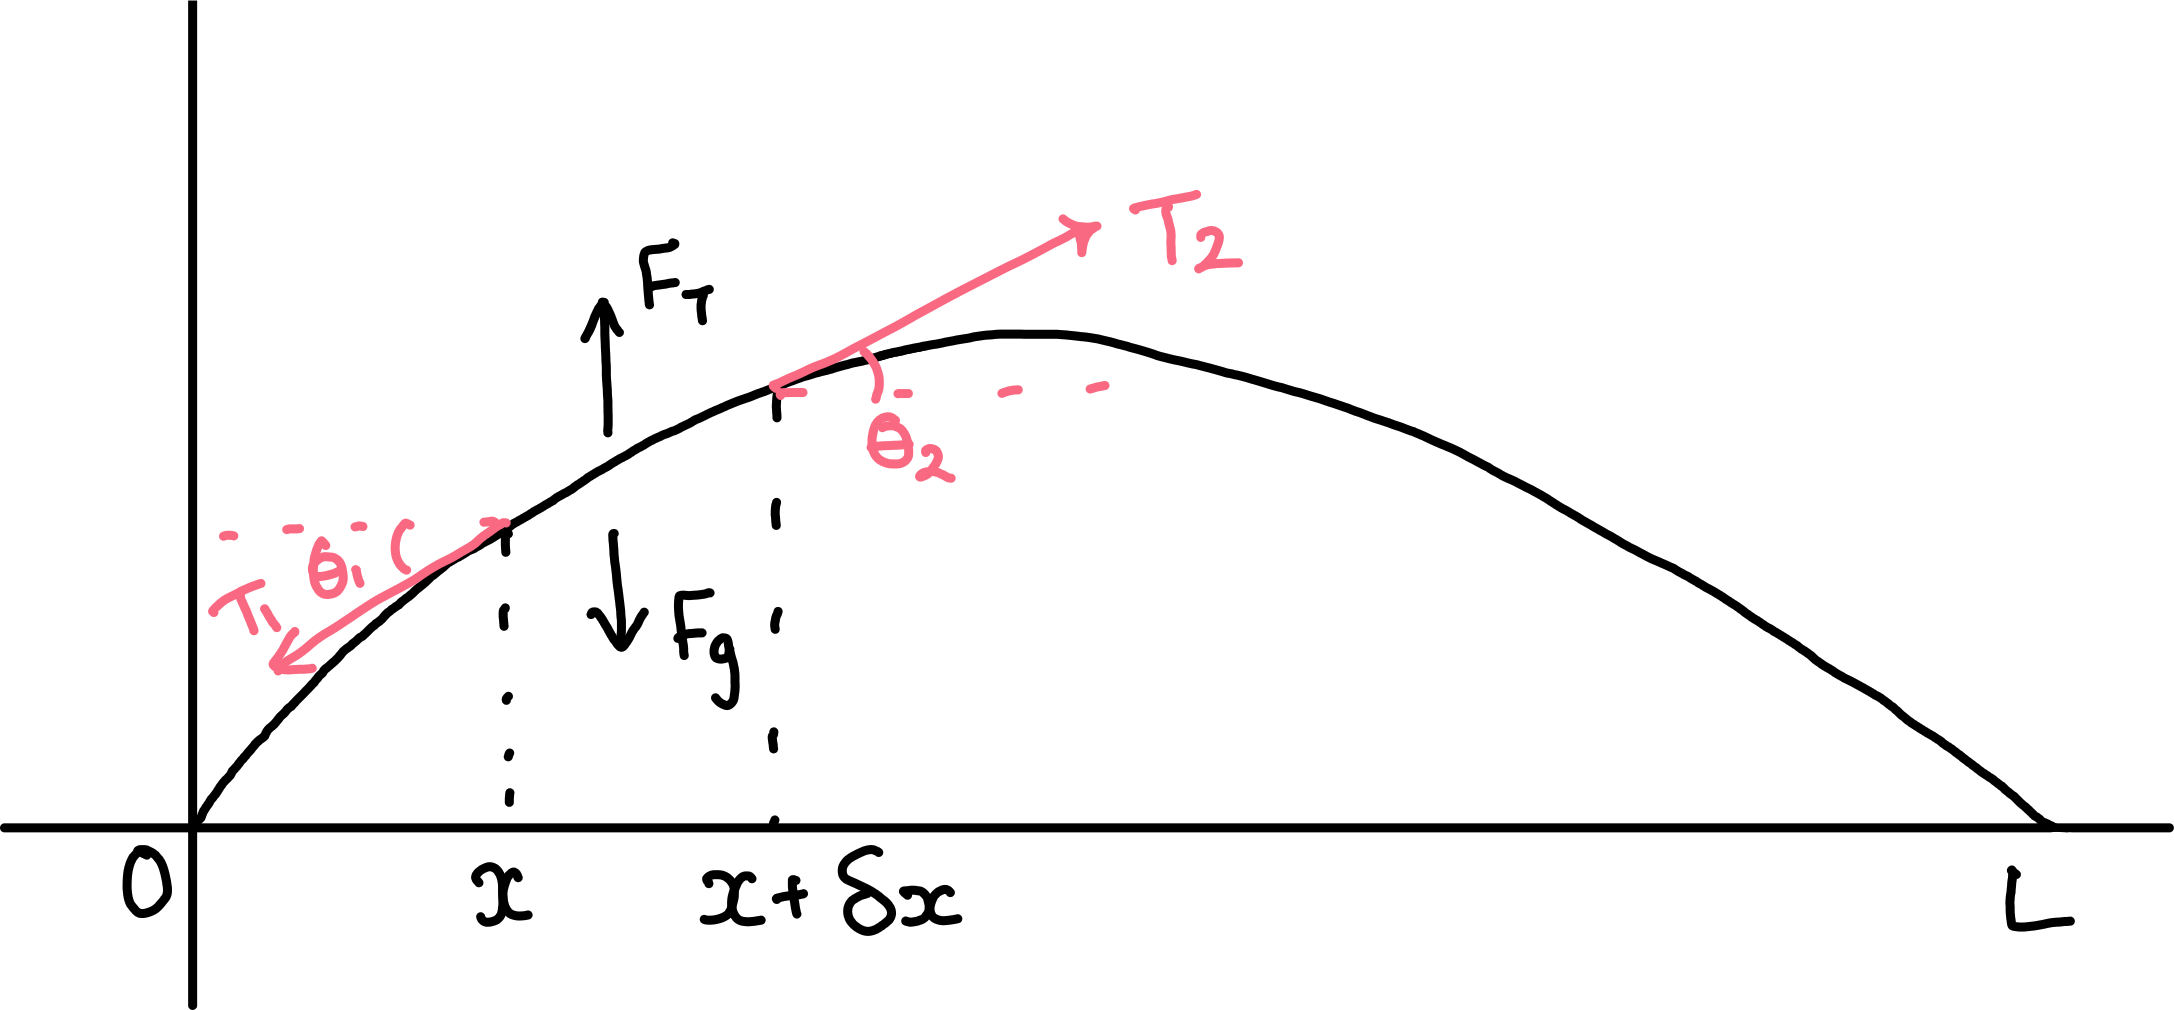
\includegraphics[height=5cm]{03-string} 
\end{figure}

Let $T_1$ be the tension force acting to the left at angle $\theta_1$ from the horizontal.
Analogously, let $T_2$ be the rightwards tension force at angle $\theta_2$.
We assume at any point on the string that $\abs{\pdv{y}{x}} \ll 1$, so the angles of the forces, $\theta_1, \theta_2$ are small.
In the $x$ dimension,
\begin{align*}
	T_1 \cos \theta_1 = T_2 \cos \theta_2 \implies T_1 \approx T_2 = T \text{ by small angle approximation}
\end{align*}
So the tension $T$ is a constant independent of $x$ up to an error of order $O\qty(\abs{\pdv{y}{x}
}^2)$.
In the $y$ dimension, since the $\theta$ are small,
\begin{align*}
	F_T = T_2 \sin \theta_2 - T_1 \sin \theta_1 \approx T \qty(\eval{\pdv{y}{x}}_{x + \delta x} - \eval{\pdv{y}{x}}_x) \approx T \pdv[2]{y}{x} \delta x
\end{align*}
By $F = ma$,
\begin{align*}
	F_T + F_g = (\mu \, \delta x) \pdv[2]{y}{t} = T \pdv[2]{y}{x} \delta x - g \mu \delta x
\end{align*}
where $F_g$ is the gravitational force and $\mu$ is the mass per unit length (linear mass density).
We define the wave speed as
\begin{align*}
	c = \sqrt{\frac{T}{\mu}} \text{ (a constant)}
\end{align*}
and find
\begin{align}
	\pdv[2]{y}{t} = \frac{T}{\mu} \pdv[2]{y}{x} - g = c^2 \pdv[2]{y}{x} - g \label{eq:3.3}
\end{align}
We often assume gravity is negligible to produce the pure wave equation
\begin{align} \label{eq:3.4}
	\frac{1}{c^2} \pdv[2]{y}{t} = \pdv[2]{y}{x}.
\end{align}
The 1D wave equation is then $\ddot{y} = c^2 y''$.

\subsection{Separation of variables}
We wish to solve the wave equation \cref{eq:3.4} subject to  boundary conditions \cref{eq:3.1} and initial conditions \cref{eq:3.2}.
Consider a possible solution of \underline{seperable form} (ansatz):
\begin{align} \label{eq:3.5}
	y(x,t) = X(x) T(t)
\end{align}
Substituting into the wave equation \cref{eq:3.4},
\begin{align*}
	\frac{1}{c^2} \ddot y = y'' \implies \frac{1}{c^2} X \ddot T = X'' T.
\end{align*}
Then
\begin{align*}
	\frac{1}{c^2}\frac{\ddot T}{T} = \frac{X''}{X}
\end{align*}
However, $\frac{\ddot T}{T}$ depends only on $t$ and $\frac{X''}{X}$ depends only on $x$.
Thus, both sides must be equal to some \textit{separation constant} $-\lambda$.
\begin{align*}
	\frac{1}{c^2}\frac{\ddot T}{T} = \frac{X''}{X} = -\lambda
\end{align*}
Hence,
\begin{align}
	X'' + \lambda X &= 0 \label{eq:3.6} \\ 
	\ddot T + \lambda c^2 T &= 0. \label{eq:3.7}
\end{align}

\subsection{Boundary conditions and normal modes}
We will begin by first solving the spatial ODE \cref{eq:3.6}.
One of $\lambda > 0, \lambda < 0, \lambda = 0$ must be true.
The boundary conditions \cref{eq:3.1} restrict the possible $\lambda$.
\begin{enumerate}
	\item First, suppose $\lambda < 0$.
	      Take $\chi^2 = -\lambda$.
	      Then,
	      \begin{align*}
		      X(x) = Ae^{\chi x} + Be^{-\chi x} = \tilde A \cosh (\chi x) + \tilde B \sinh (\chi x).
	      \end{align*}
	      The boundary conditions are $x(0) = x(L) = 0$, so only the trivial solution is possible: $\tilde A = \tilde B = 0$.
	\item Now, suppose $\lambda = 0$.
	      Then
	      \begin{align*}
		      X(x) = Ax + B.
	      \end{align*}
	      Again, the boundary conditions impose $A = B = 0$ giving only the trivial solution.
	\item Finally, the last possibility is $\lambda > 0$.
	      \begin{align*}
		      X(x) = A \cos \qty(\sqrt{\lambda} x) + B \sin \qty(\sqrt{\lambda} x)
	      \end{align*}
	      The boundary conditions give
	      \begin{align*}
		      A = 0;\quad B \sin \qty(\sqrt{\lambda} L) = 0 \implies \sqrt{\lambda} L = n \pi.
	      \end{align*}
		  The following are the eigenfunctions and eigenvalues.
		\begin{align}
			X_n(x) = B_n \sin \frac{n \pi x}{L};\quad \lambda_n = \qty(\frac{n \pi}{L})^2 \ (n > 0) \label{eq:3.8}
		\end{align}
\end{enumerate}

These are also called the \vocab{normal modes} of the system because the spatial shape in $x$ does not change in time, but the amplitude may vary. \\
The fundamental mode is the lowest frequency of vibration, given by
\begin{align*}
	n = 1 \implies \lambda_1 = \frac{\pi^2}{L^2}
\end{align*}
\begin{figure}[h] 
    \centering 
    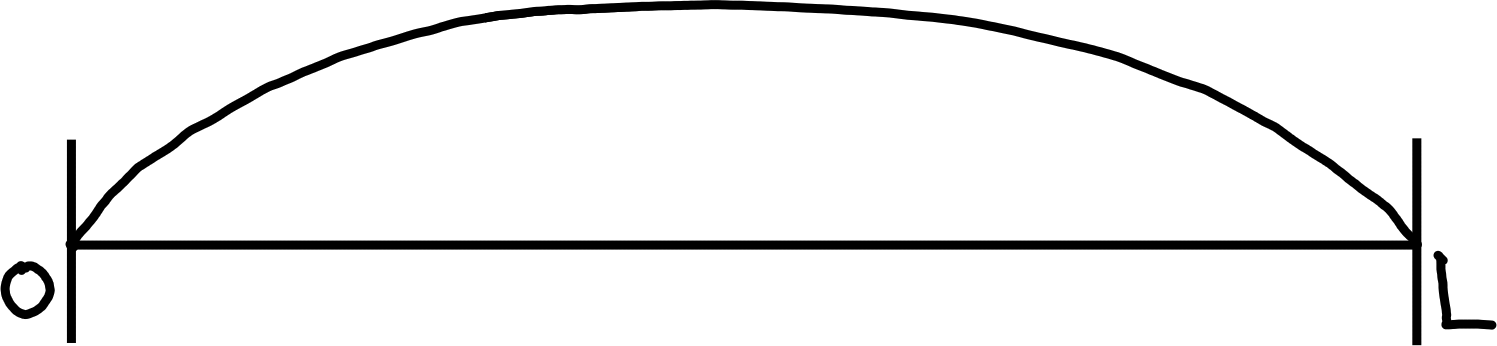
\includegraphics[height=5cm]{03-firstharmonic} 
\end{figure}
The second mode is the first overtone, and is given by
\begin{align*}
	n = 2 \implies \lambda_2 = \frac{4\pi^2}{L^2}
\end{align*}
\begin{figure}[h] 
    \centering 
    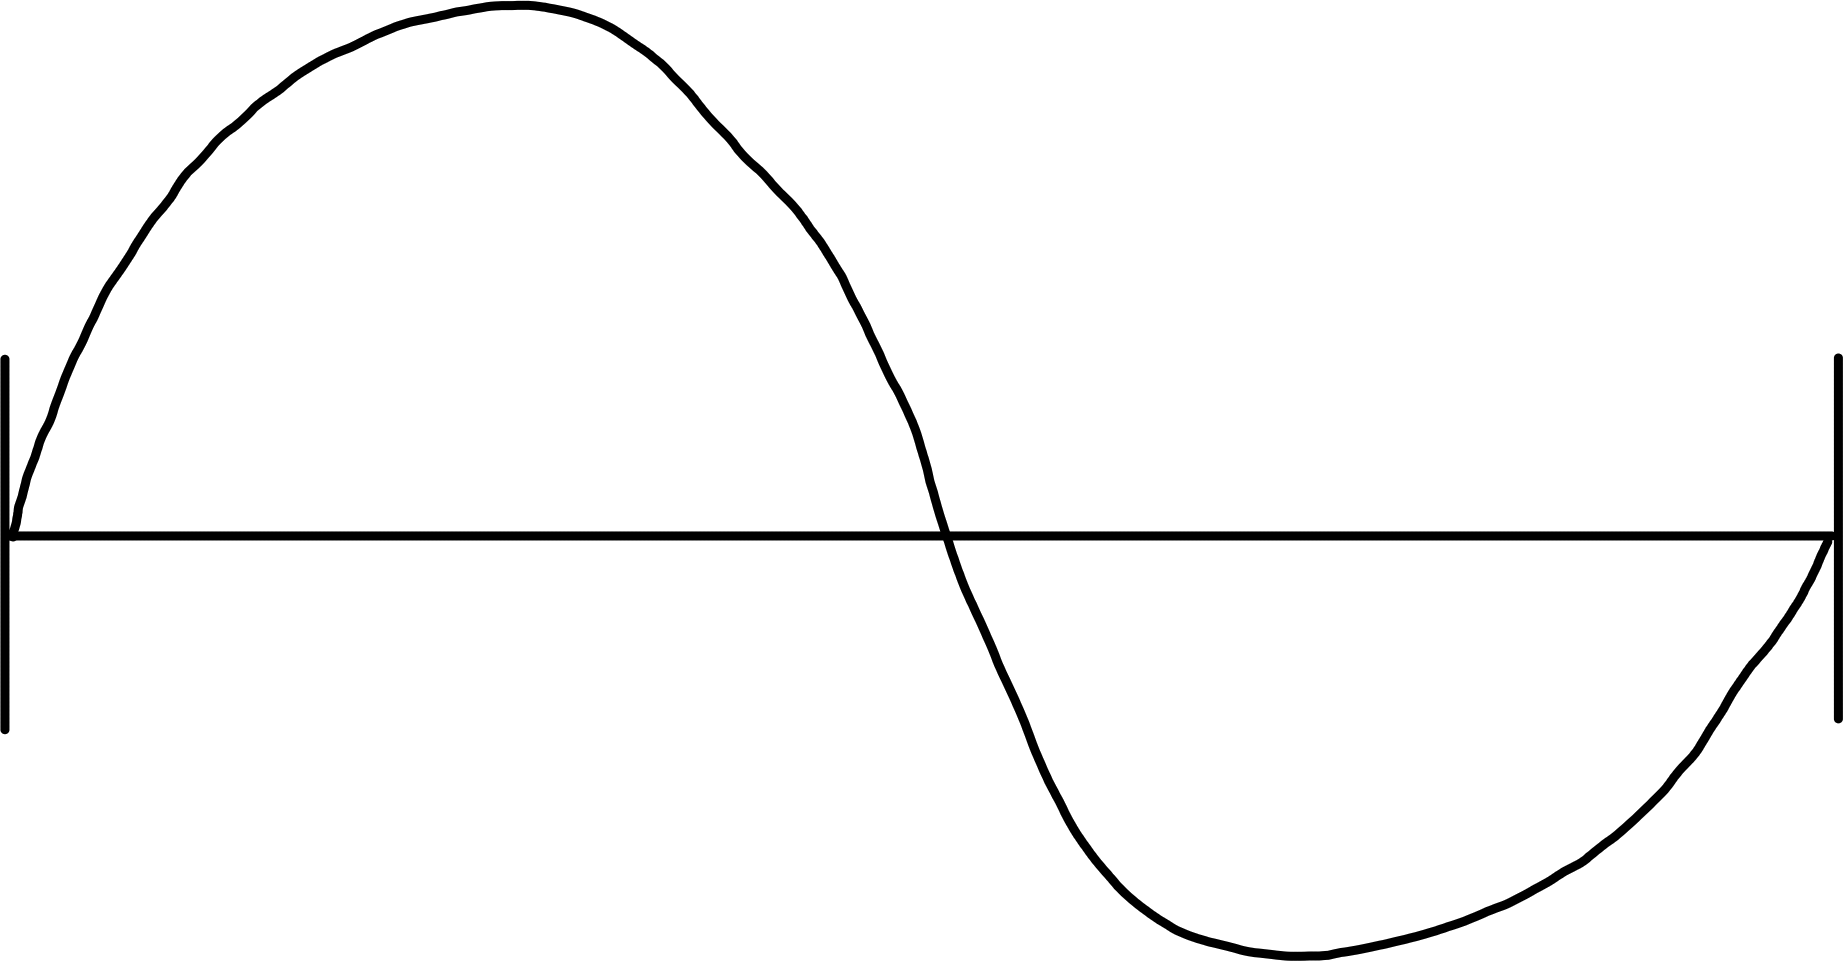
\includegraphics[height=5cm]{03-secondharmonic} 
\end{figure}

\subsection{Initial conditions and temporal solutions}
Substituting $\lambda_n$ into the time ODE \cref{eq:3.7},
\begin{align*}
	\ddot T + \frac{n^2 \pi^2 c^2}{L^2}T = 0.
\end{align*}
Hence,
\begin{align} \label{eq:3.9}
	T_n(t) = C_n \cos \frac{n \pi c t}{L} + D_n \sin \frac{n \pi c t}{L}.
\end{align}

Therefore, a specific solution of the wave equation, \cref{eq:3.4}, satisfying the boundary conditions, \cref{eq:3.1}, is (absorbing the $B_n$ into the $C_n, D_n$):
\begin{align*}
	y_n(x,t) = T_n(t) X_n(x) = \qty(C_n \cos \frac{n \pi c t}{L} + D_n \sin \frac{n \pi c t}{L}) \sin \frac{n \pi x}{L}
\end{align*}

\begin{exercise}
	Verify it's a solution.
\end{exercise} 

Since the wave equation \cref{eq:3.4} is linear (and b.c.s \cref{eq:3.1} are homogenous) we can add the solutions (the $y_n$) together to find \vocab{general string solution}
% To find a particular solution for a given set of initial conditions, we must consider a linear superposition of all possible $y_n$.
\begin{align} \label{eq:3.10}
	y(x,t) = \sum_{n=1}^\infty \qty(C_n \cos \frac{n \pi c t}{L} + D_n \sin \frac{n \pi c t}{L}) \sin \frac{n \pi x}{L}.
\end{align}
By construction, this $y(x,t)$ satisfies the boundary conditions, so now we can impose the initial conditions \cref{eq:3.2}:
\begin{align*}
	y(x,0) = p(x) = \sum_{n=1}^\infty C_n \sin \frac{n \pi x}{L}
\end{align*}
We can find the $C_n$ using standard Fourier series techniques \cref{eq:1.12}, since this is exactly a half-range sine series.
Further,
\begin{align*}
	\pdv{y(x,0)}{t} = q(x) = \sum_{n=1}^\infty \frac{n \pi c}{L} D_n \sin \frac{n \pi x}{L}
\end{align*}
Again we can solve for the $D_n$ in a similar way.
Using \cref{eq:1.12}:
\begin{align}
	\begin{aligned} \label{eq:3.11}
		C_n &= \frac{2}{L} \int_0^L p(x) \sin \frac{n \pi x}{L} \dd{x} \\
		D_n &= \frac{2}{n \pi c} \int_0^L q(x) \sin \frac{n \pi x}{L} \dd{x}
	\end{aligned}
\end{align} 

Hence \cref{eq:3.11} is the solution to \cref{eq:3.4} satisfying \cref{eq:3.1,eq:3.2}.

\begin{example}
	Consider the initial condition of a see-saw wave parametrised by $\xi$, and let $L = 1$.
	This can be visualised as plucking the string at position $\xi$.
	\begin{align*}
		y(x,0) = p(x) = \begin{cases}
			x(1-\xi) & 0 \leq x < \xi \\
			\xi(1-x) & \xi \leq x < 1
		\end{cases}
	\end{align*}
	We also define
	\begin{align*}
		\pdv{y(x,0)}{t} = q(x) = 0
	\end{align*}
	The Fourier series \cref{eq:1.8} for $p$ is given by
	\begin{align*}
		C_n = \frac{2 \sin n \pi \xi}{(n \pi)^2};\quad D_n = 0
	\end{align*}
	Hence the solution to the wave equation is
	\begin{align*}
		y(x,t) = \sum_{n=1}^\infty \frac{2}{(n \pi)^2} \sin n \pi \xi \sin n \pi x \cos n \pi c t
	\end{align*}
	Take $\xi = \frac{1}{2}, C_{2m} = 0, C_{2m - 1} = \frac{2 (-1)^{m + 1}}{((2m-1) \pi)^2}$ (odd only), e.g. Guitar has $\frac{1}{4} \leq \xi \leq \frac{1}{3}$, Violin $\xi \approx \frac{1}{7}$.
\end{example}

\begin{aside}{Solution in characterstic coordinates}
	Recall sine/cosine summation identities (before \cref{eq:1.1}) which means our general solution \cref{eq:3.10} becomes
	\begin{align}
		y(x, t) &= \frac{1}{2} \sum_{n=1}^{\infty} \qty[C_n \sin \frac{n \pi}{L} (x-ct) + D_n \cos \frac{n \pi}{L} (x - ct) + C_n \sin \frac{n \pi}{L} (x + ct) + D_n \cos \frac{n \pi}{L} (x + ct)] \notag \\
		&\equiv f(x - ct) + g(x + ct) \label{eq:3.12}
	\end{align} 
	The standing wave solution \cref{eq:3.10} is made up of a right-moving wave (along characteristic $x - ct = \eta$, $\eta$ a constant) and a left-moving wave ($x + ct = \xi$, $\xi$ a constant) i.e. a general solution with arbitrary $f, g$ (see later).

	\underline{Special case}: $q(x) = 0$ in \cref{eq:3.1} $\implies f = g = \frac{1}{2} D$ at $t = 0$.
	\begin{figure}[h] 
		\centering 
		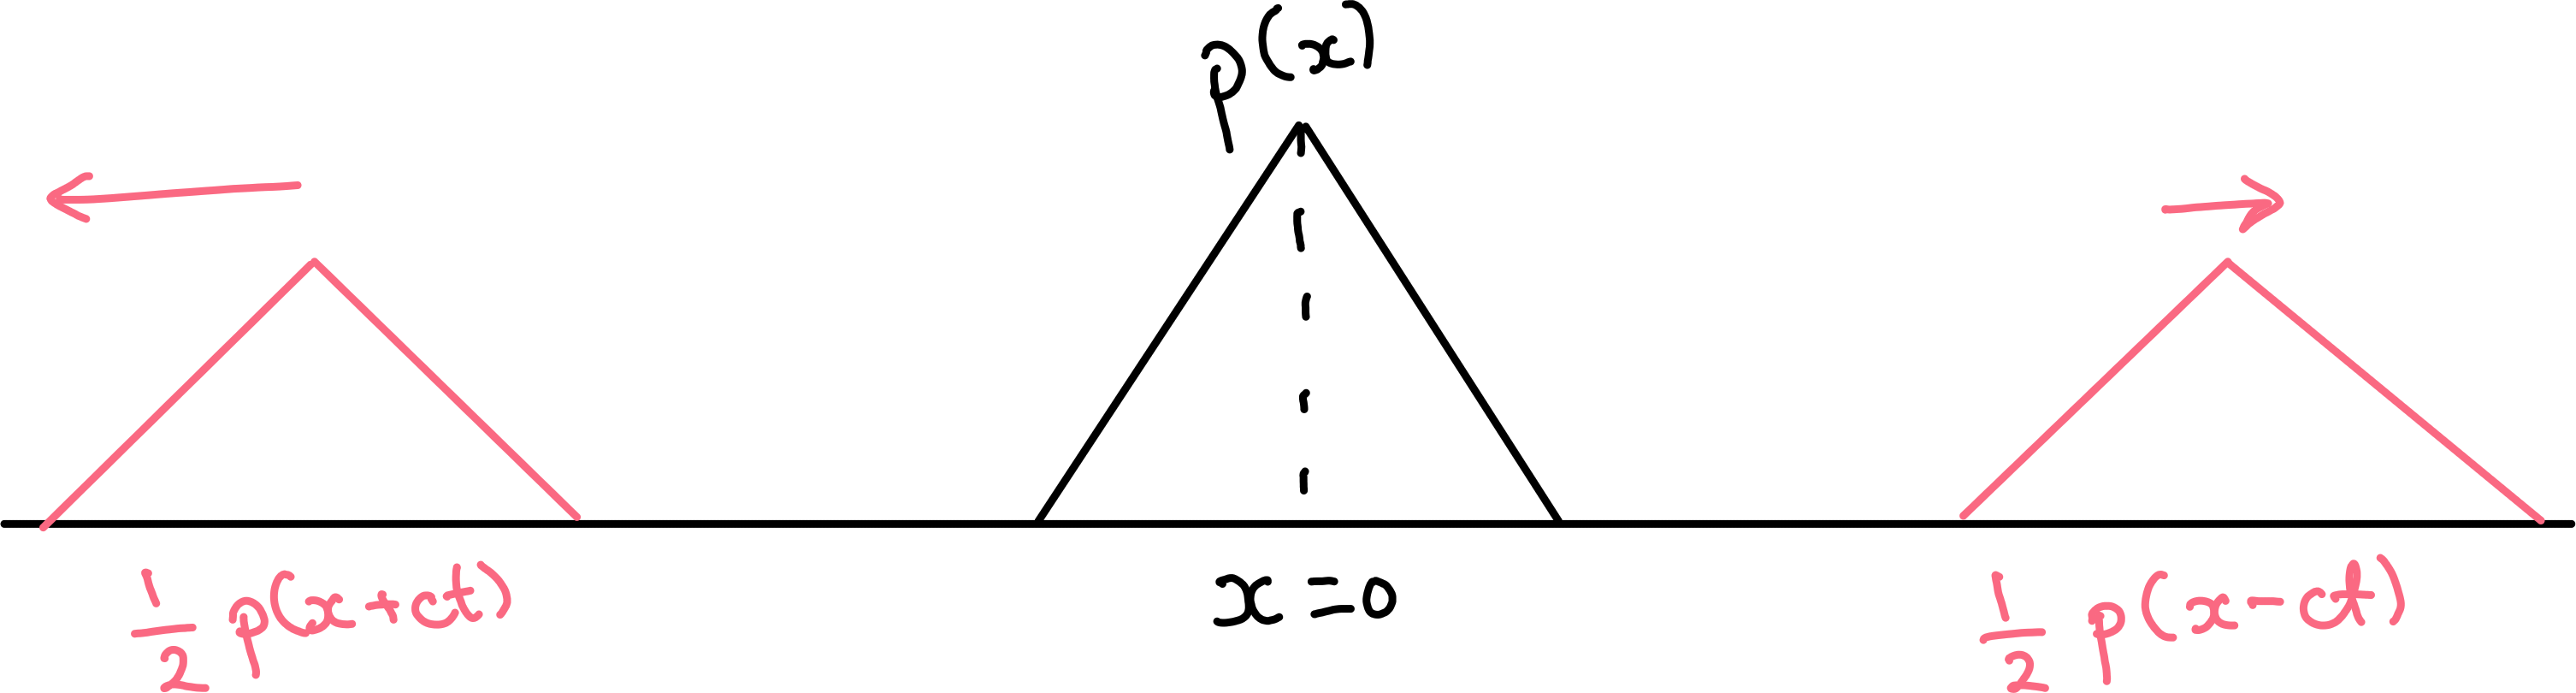
\includegraphics[height=5cm]{03-specialcase} 
	\end{figure}
	
\end{aside} 

\subsection{Separation of variables methodology}
A general strategy for solving higher-dimensional partial differential equations is as follows.
\begin{enumerate}
	\item Obtain a linear PDE system, using boundary and initial conditions.
	\item Separate variables to yield decoupled ODEs.
	\item Impose homogeneous boundary conditions to find eigenvalues and eigenfunctions.
	\item Use these eigenvalues (constants of separation) to find the eigenfunctions in the other variables.
	\item Sum over the products of separable solutions to find the general series solution.
	\item Determine coefficients for this series using the initial conditions.
\end{enumerate}
% \begin{example}
% 	We will solve the wave equation instead in characteristic coordinates.
% 	Recall the sine and cosine summation identities:
% 	\begin{align*}
% 		y(x,t) & = \frac{1}{2} \sum_{n=1}^\infty \Bigg[ \qty(C_n \sin \frac{n \pi}{L}(x-ct) + D_n \cos \frac{n \pi}{L}(x-ct)) \\&
% 		+ \qty(C_n \sin \frac{n \pi}{L}(x+ct) - D_n \cos \frac{n \pi}{L}(x+ct)) \Bigg]                                        \\
% 		       & = f(x-ct) + g(x+ct)
% 	\end{align*}
% 	The standing wave solution can be interpreted as a superposition of a right-moving wave and a left-moving wave.
% 	A special case is $q(x) = 0$, implying $f = g = \frac{1}{2} p$.
% 	Then,
% 	\begin{align*}
% 		y(x,t) = \frac{1}{2}\qty[p(x-ct) + p(x+ct)]
% 	\end{align*}
% \end{example}

\subsection{Energy of oscillations}
A vibrating string has kinetic energy due to its motion.
\begin{align*}
	\text{Kinetic energy} = \frac{1}{2} \mu \int_0^L \qty(\pdv{y}{t})^2 \dd{x}
\end{align*}
It has potential energy  due to stretching by $\Delta x$ given by
\begin{align*}
	\text{Potential energy} = T \Delta x = T \int_c^T \qty(\underbrace{\sqrt{1 + \qty(\pdv{y}{x})^2}}_\text{arc length $s$} -1)\dd{x} \approx \frac{1}{2} T \int_0^L \qty(\pdv{y}{x})^2 \dd{x}
\end{align*}
assuming that the disturbances on the string are small, that is, $\abs{\pdv{y}{x}} \ll 1$.
The total energy on the string, given $c^2 = T/\mu$, is given by
\begin{align} \label{eq:3.13}
	E = \frac{1}{2}\mu \int_0^L \qty[\qty(\pdv{y}{t})^2 + c^2 \qty(\pdv{y}{x})^2] \dd{x}
\end{align}
Substituting the solution \cref{eq:3.10}, using the orthogonality conditions \cref{eq:1.1},
\begin{align}
	E &= \frac{1}{2}\mu \sum_{n=1}^\infty \int_0^L \Bigg[\qty(-\frac{n \pi c}{L} C_n \sin \frac{n \pi c t}{L} + \frac{n \pi c}{L} D_n \cos \frac{n \pi c t}{L})^2 \sin^2 \frac{n \pi x}{L}\notag \\
	&+ c^2 \qty(C_n \cos \frac{n \pi c t}{L} + D_n \sin \frac{n \pi c t}{L})^2 \frac{n^2 \pi^2}{L^2} \cos^2 \frac{n \pi x}{L} \Bigg] \dd{x} \notag \\
	&= \frac{1}{4} \mu \sum_{n=1}^\infty \frac{n^2 \pi^2 c^2}{L} \qty(C_n^2 + D_n^2) \label{eq:3.14}
\end{align}
which is an analogous result to Parseval's theorem.
This is true since \begin{align*}
	\int \cos^2 \frac{n \pi x}{L}\dd{x} = \frac{1}{2}
\end{align*} and $\cos^2 + \sin^2 = 1$.
We can think of this energy as the sum over all the normal modes of the energy in that specific mode.
Note that this quantity is constant over time (no dissipation).

\subsection{Wave reflection and transmission}
Recall the travelling wave solution \cref{eq:3.12}.
The travelling wave has left-moving and right-moving modes.
A \vocab{simple harmonic} travelling wave is
\begin{align*}
	y = \Re\qty[ A e^{i \omega(t-x/c)} ] = A \cos \qty[\omega(t-x/c) + \phi]
\end{align*}
where the phase $\phi$ is equal to $\arg A$, and the wavelength $\lambda$ is $2 \pi c / \omega$.
In further discussion, we assume only the real part is used.

Consider a density discontinuity on the string at $x = 0$ with the following properties.
\begin{align*}
	\mu = \begin{cases}
		\mu_- & \text{for } x < 0 \\
		\mu_+ & \text{for } x > 0
	\end{cases} \implies c = \begin{cases}
		c_- = \sqrt{\frac{T}{\mu_-}} & \text{for } x < 0 \\
		c_+ = \sqrt{\frac{T}{\mu_+}} & \text{for } x > 0 \\
	\end{cases}
\end{align*}
assuming a constant tension $T$.
As a wave from the negative direction approaches the discontinuity, some of the wave will be reflected, given by $B e^{i \omega(t + x/c_-)}$, and some of the wave will be transmitted, given by $D e^{i \omega(t - x/c_+)}$.
\begin{figure}[h] 
    \centering 
    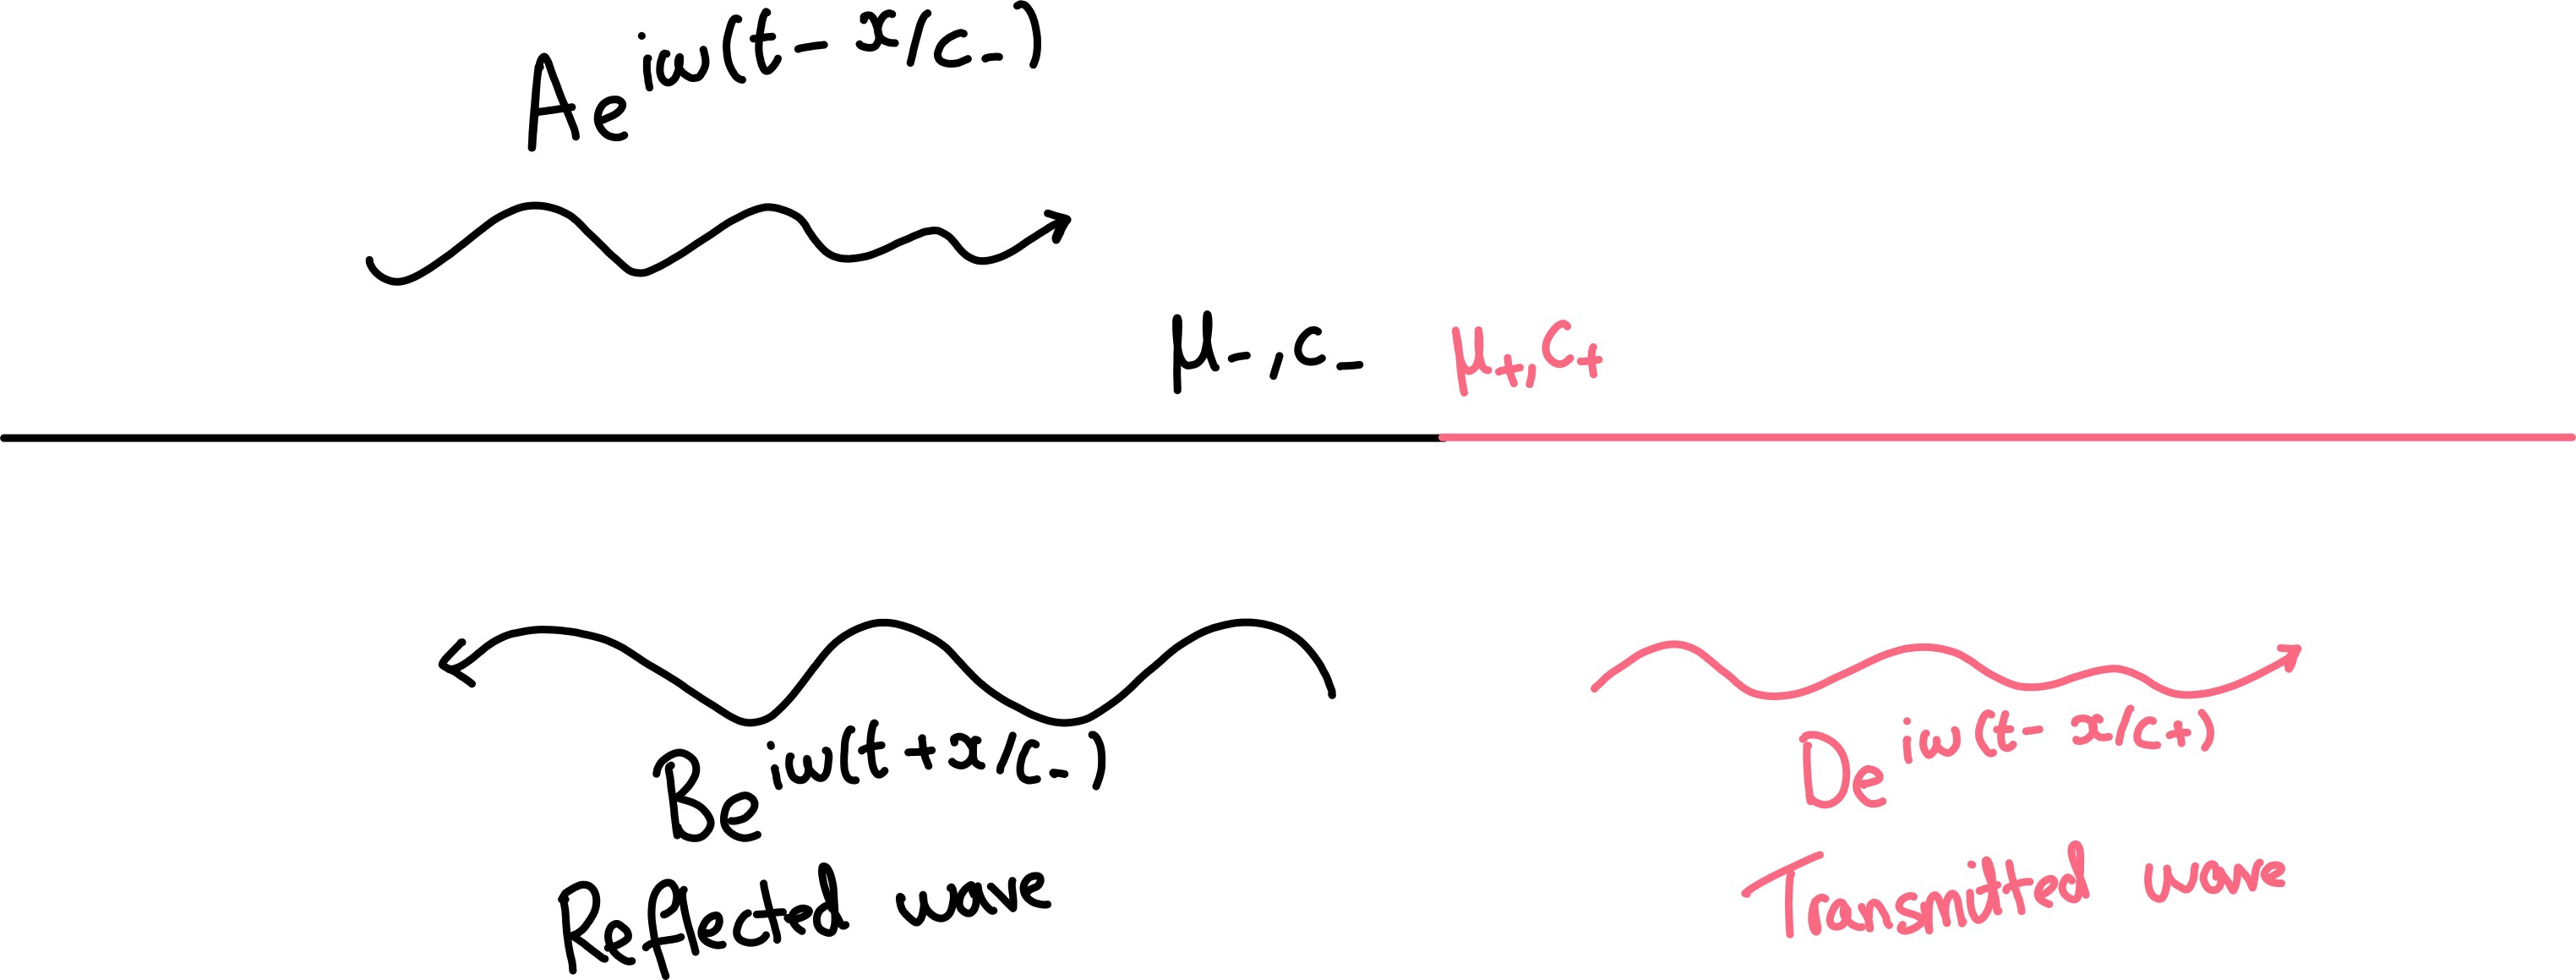
\includegraphics[height=5cm]{03-densitydiscon} 
\end{figure}
The boundary conditions at $x = 0$ are
\begin{enumerate}
	\item $y$ is continuous for all $t$ (the string does not break), so
	\begin{equation}
		A + B = D \tag{$\ast$}
	\end{equation}
	\item The forces balance, $T \eval{\pdv{y}{x}}_{x = 0^-} = T \eval{\pdv{y}{x}}_{x = 0^+}$ which means $\pdv{y}{x}$ must be continuous for all $t$.
	This gives
	\begin{equation}
		\frac{-i\omega A}{c_-} + \frac{i \omega B}{c_-} = \frac{-i \omega D}{c_+} \tag{$\dagger$}
	\end{equation}
\end{enumerate}
We can eliminate $B$ from $(\ast)$ by subtracting $\frac{c_-}{i \omega}(\dagger)$.
\begin{align*}
	2A = D + D \frac{c_-}{c_+} = \frac{D}{c_+}(c_+ + c_-)
\end{align*}
Hence, given $A$, we have the solution for the transmitted amplitude and reflected amplitude to be
\setcounter{equation}{15}
\begin{align} \label{eq:3.16}
	D = \frac{2 c_+}{c_- + c_+} A;\quad B = \frac{c_+ - c_-}{c_- + c_+}
\end{align}
In general $A, B, D$ are complex, hence different phase shifts are possible.

There are a number of limiting cases, for example
\begin{enumerate}
	\item If $c_- = c_+$ we have $D = A$ and $B = 0$ so we have full transmission and no reflection.
	\item (Dirichlet boundary conditions) If $\frac{\mu_+}{\mu_-} \to \infty$, this models a fixed end at $x = 0$.
	      We have $\frac{c_+}{c_-} \to 0$ giving $D = 0$ and $B = -A$.
	      Notice that the reflection has occurred with opposite phase, $\phi = \pi$.
	\item (Neumann boundary conditions) Consider $\frac{\mu_+}{\mu_-} \to 0$, this models a free end.
	      Then $\frac{c_+}{c_-} \to \infty$ giving $D = 2A$, $B = A$.
	      This gives total reflection but with the same phase.
\end{enumerate}

\subsection{Wave equation in 2D plane polar coordinates}
Consider the two-dimensional wave equation for $u(r,\theta,t)$ given by
\begin{align} \label{eq:3.17}
	\frac{1}{c^2} \pdv[2]{u}{t} = \laplacian u
\end{align}
with boundary conditions at $r = 1$ on a unit disc given by
\begin{align} \label{eq:3.18}
	u(1,\theta,t) = 0 \quad \text{(fixed rim)}
\end{align}
and initial conditions for $t = 0$ given by
\begin{align} \label{eq:3.19}
	u(r,\theta,0) = \phi(r,\theta);\quad \pdv{u}{t}(r,\theta,0) = \psi(r,\theta)
\end{align}

\subsubsection{Temporal Seperation}
Suppose that this equation is separable.
First, let us consider temporal separation.
Suppose that
\begin{align} \label{eq:3.20}
	u(r,\theta,t) = T(t) V(r,\theta)
\end{align}
Then substitute into \cref{eq:3.17}
\begin{align}
	\ddot T + \lambda c^2 T &= 0 \label{eq:3.21} \\
	\laplacian V + \lambda V &= 0 \label{eq:3.22}
\end{align}
In plane polar coordinates, we can write the spatial equation \cref{eq:3.22} as
\begin{align*}
	\pdv[2]{V}{r} + \frac{1}{r} \pdv{V}{r} + \frac{1}{r^2}\pdv[2]{V}{\theta} + \lambda V = 0
\end{align*}
\subsubsection{Spatial Seperation}
We will perform another separation, supposing
\begin{align*}
	V(r,\theta) = R(r) \Theta(\theta).
\end{align*}
Substitute into \cref{eq:3.22}
\begin{align}
	\Theta'' + \mu \Theta &= 0 \label{eq:3.23} \\
	r^2 R'' + r R' + \qty(\lambda r^2 - \mu) R &= 0 \label{eq:3.24}
\end{align}
where $\lambda, \mu$ are the separation constants.
\subsubsection{Polar Solution}
The polar solution is constrained by periodicity $\Theta(0) = \Theta(2 \pi)$, since we are working on a disc.
We also consider only $\mu > 0$.
The eigenvalue is then given by $\mu = m^2$, where $m \in \mathbb N \cup \{0\}$.
\begin{align} \label{eq:3.25}
	\Theta_m(\theta) = A_m \cos m \theta + B_m \sin m \theta
\end{align}
Or, in complex exponential form,
\begin{align*}
	\Theta_m(\theta) = C_m e^{im\theta};\quad m \in \mathbb Z
\end{align*}

\subsection{Radial Equations}
We can solve the radial equation \cref{eq:3.24} (in the previous subsection) by converting it first into Sturm-Liouville form \cref{eq:2.7}, which can be accomplished by dividing by $r$ with $\mu = m^2$.
\begin{align} \label{eq:3.26}
	\dv{r} \qty(r R') - \frac{m^2}{r} = -\lambda r R \quad (0 \leq r \leq 1)
\end{align}
where $p(r) = r, q(r) = \frac{m^2}{r}, w(r) = r$, with self-adjoint boundary conditions with $R(1) = 0$.
We will require $R$ is bounded at $R(0)$, and since $p(0) = 0$ there is a regular singular point at $r = 0$.

\subsubsection{Bessel's equation}
This particular equation for $R$ is known as Bessel's equation.
We will first substitute $z \equiv \sqrt{\lambda} r$ in \cref{eq:3.26}, then we find the usual form of Bessel's equation\footnote{May also be written as $(z R')' + (z - m^2 / z) R = 0$},
\begin{align} \label{eq:3.27}
	z^2 \dv[2]{R}{z} + z \dv{R}{z} + (z^2 - m^2)R = 0
\end{align}

\subsubsection{Frobenius Solution}
We can use the method of Frobenius by substituting the following power series:
\begin{align*}
	R = z^p \sum_{n=0}^\infty a_n z^n
\end{align*}
to find
\begin{align*}
	\sum_{n=0}^\infty \qty[ a_n (n+p)(n+p-1) z^{n+p} + (n+p) z^{n+p} + z^{n+p+2} + m^2 z^{n+p} ] = 0
\end{align*}
Equating powers of $z$, we can find the indicial equation
\begin{align*}
	p^2 - m^2 = 0 \implies p = m, -m
\end{align*}
The regular solution, given by $p = m$, has recursion relation
\begin{align*}
	(n+m)^2 a_n + a_{n-2} - m^2 a_n = 0
\end{align*}
which gives
\begin{align*}
	a_n = \frac{-1}{n(n+2m)} a_{n-2}
\end{align*}
Hence, we can find
\begin{align*}
	a_{2n} = a_0 \frac{(-1)^n}{2^{2n} n!
		(n+m)(n+m-1) \dots (m+1)}
\end{align*}
If, by convention, we let
\begin{align*}
	a_0 = \frac{1}{2^m m!}
\end{align*}
we can then write the \textit{Bessel function of the first kind} by
\begin{align} \label{eq:3.28}
	J_m(z) = \qty(\frac{z}{2})^m \sum_{n=0}^\infty \frac{(-1)^n}{n!
		(n+m)!} \qty(\frac{z}{2})^{2n}
\end{align}

\begin{exercise}
	Use $y = \sqrt{z} R$ in Bessel's eqn \cref{eq:3.27} to find $y'' + y (1 + \frac{1}{4z} - \frac{m^2}{z^2})$.
	So, as $z \to \infty$, $y'' = -y$ so we have solns $R = \frac{1}{\sqrt{z}} (A \cos z + B \sin z)$.
\end{exercise}

Also works for $m = \mu$ ($\mu \notin \mathbb{Z}$) if $(n + m)! \to \Gamma(n + m + 1)$.
Second soln with $p = -m$ (integer) is the Neuman function (Bessel function of second kind).
\begin{align*}
	Y_m(z) = \lim_{\mu \to m} \frac{J_\mu \cos(\mu \pi) - J_{-\mu}(z)}{\sin \mu \pi}
\end{align*} 

\begin{exercise}
	Use \cref{eq:3.28} to show that $\frac{d}{dz} (z^m J_m(z)) = z^m J_{m-1}(z)$ and hence
	\begin{align} \label{eq:3.29}
		J'_m(z) + \frac{m}{z} J_m(z) = J_{m-1}(z)
	\end{align}
	Repeat with $z^{-m}$ to find \underline{recursion relations}
	\begin{align} \label{eq:3.30}
		\begin{aligned}
			J_{m-1}(z) + J_{m+1}(z) &= \frac{2m}{z} J_m(z) \\
			J_{m-1}(z) - J_{m+1}(z) &= 2 J'_m(z)
		\end{aligned}
	\end{align} 
\end{exercise} 

\subsection{Asymptotic behaviour of Bessel functions}
If $z$ is small, the leading-order behaviour of $J_m(z)$ is
\begin{align}
	J_0(z) & \approx 1 \notag \\
	J_m(z) & \approx \frac{1}{m!} \qty(\frac{z}{2})^m \notag \\
	Y_0(z) &\to \frac{2}{\pi} \ln(\frac{z}{2}) \notag \\
	Y_m(z) &\to - \frac{(m-1)!}{\pi} (\frac{2}{z})^m \label{eq:3.31}
\end{align}
Now, let us consider large $z$.
In this case, the function becomes oscillatory;
\begin{align}
	J_m(z) &\approx \sqrt{\frac{2}{\pi z}} \cos(z - \frac{m \pi}{2} - \frac{\pi}{4}) \label{eq:3.32} \\
	Y_m(z) &\approx \sqrt{\frac{2}{\pi z}} \sin(z - \frac{m \pi}{2} - \frac{\pi}{4}) \notag
\end{align}

\subsection{Zeroes of Bessel functions $J_m(z)$}
We can see from the asymptotic behaviour that there are infinitely many zeroes of the Bessel functions of the first kind as $z \to \infty$.
We define $j_{mn}$ to be the $n$th zero of $J_m$, for $z > 0$.
Approximately using \cref{eq:3.32},
\begin{align*}
	\cos(z - \frac{m \pi}{2} - \frac{\pi}{4}) = 0 \implies z - \frac{m \pi}{2} - \frac{\pi}{4} = n \pi - \frac{\pi}{2} \quad \text{(modal point)}
\end{align*}
Hence
\begin{align*}
	z \approx n \pi + \frac{m \pi}{2} - \frac{\pi}{4} \equiv \widetilde j_{mn}
\end{align*}

\begin{aside}{Non-examinable}
	Accuracy, 
	\begin{align} \label{eq:3.33}
		\qty| \frac{j_{mn} - \widetilde j_{mn}}{j_{mn}} | < \frac{0.1}{n} \text{ for } n > \frac{m^2}{2}.
	\end{align}
\end{aside} 

For $J_0(z)$ actual values are $J_{01} = 2.405$, $j_{02} = 5.520$, $j_{03} = 8.653$, $j_{0n} = n \pi - \frac{\pi}{4}$ (precision $\approx 1\%/n$).

\begin{figure}[h] 
    \centering 
    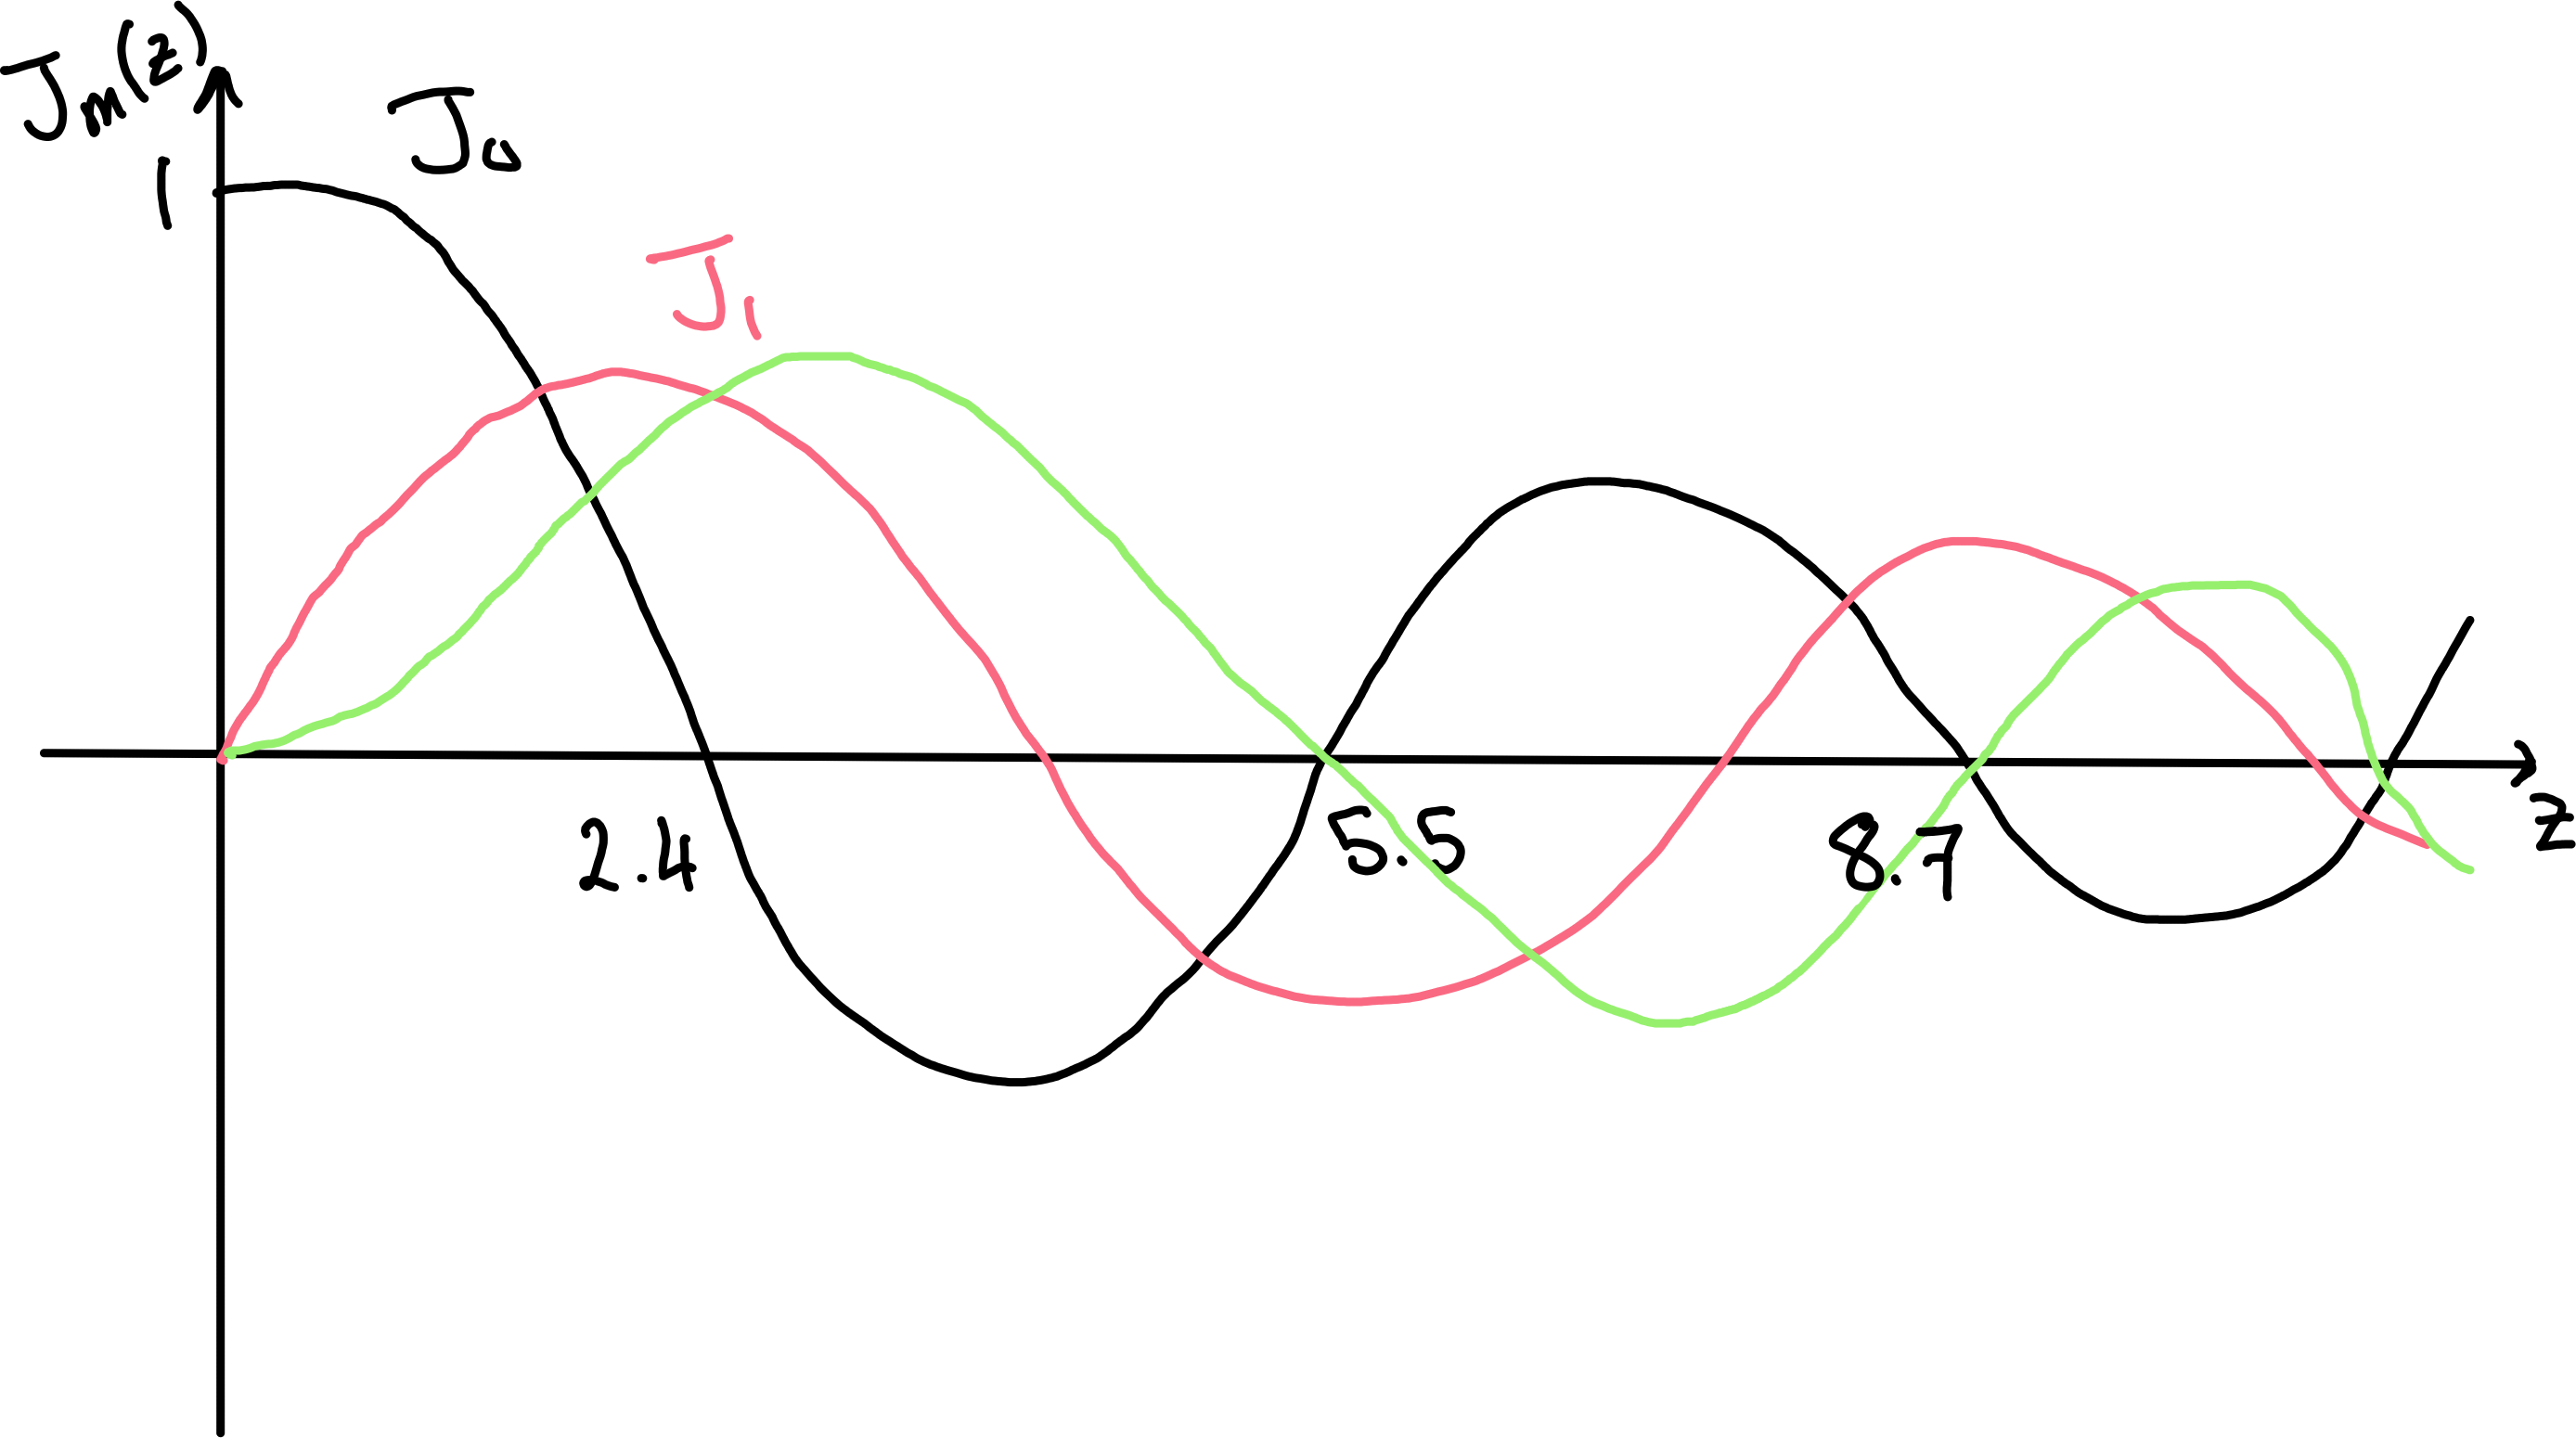
\includegraphics[height=5cm]{03-besselfunctions} 
\end{figure}

\subsection{Solving the vibrating drum}
Recall that the radial solutions to \cref{eq:3.26} become
\begin{align*}
	R_m(z) = R_m(\sqrt{\lambda} x) = A J_m(\sqrt{\lambda} x) + B Y_m(\sqrt{\lambda} x)
\end{align*}
Imposing the boundary condition of boundedness at $r = 0$, we must have $B = 0$ by \cref{eq:3.31}.
Further imposing $r = 1$ and $R = 0$ gives $J_m(\sqrt{\lambda}) = 0$.
These zeroes occur at $j_{mn} \approx n \pi + \frac{m \pi}{2} - \frac{\pi}{4}$.
Hence, the eigenvalues must be 
\begin{align} \label{eq:3.34}
	\lambda = j^2_{mn}.
\end{align}
Therefore, the spatial solution with the polar mode \cref{eq:3.26} is
\begin{align}
	V_{mn}(r, \theta) &= \Theta_m(\theta) R_{mn}(\sqrt{\lambda_{mn}} r) \notag \\
	&= (A_{mn} \cos m \theta + B_{mn} \sin m \theta) J_m (j_{mn} r) \label{eq:3.35}
\end{align}

The temporal solution \cref{eq:3.21} is
\begin{align*}
	\ddot T = -\lambda c^2 T \implies T_{mn}(t) = \cos(j_{mn} ct), \sin(j_{mn} ct)
\end{align*}

Combining everything together, the full solution to \cref{eq:3.17} is
\begin{align}
	\begin{aligned} \label{eq:3.36}
		u(r,\theta,t) & = \sum_{n=1}^\infty J_0(j_{0n} r) \qty( A_{0n}\cos j_{0n}ct + C_{0n}\sin j_{0n}ct ) \\
		&+ \sum_{m=1}^\infty \sum_{n=1}^\infty J_m (j_{mn}r) \qty( A_{mn} \cos m \theta + B_{mn} \sin m\theta ) \cos j_{mn} ct \\
		&+ \sum_{m=1}^\infty \sum_{n=1}^\infty J_m (j_{mn}r) \qty( C_{mn} \cos m \theta + D_{mn} \sin m\theta ) \sin j_{mn} ct
	\end{aligned}
\end{align} 

Now, we impose the \underline{initial conditions} \cref{eq:3.19} at $t = 0$
\begin{align} \label{eq:3.37}
	u(r,\theta,0) = \phi(r,\theta) = \sum_{m=0}^\infty \sum_{n=1}^\infty J_m (j_{mn}r) \qty( A_{mn} \cos m \theta + B_{mn} \sin m\theta )
\end{align}
and
\begin{align*}
	\pdv{u}{t}\qty(r,\theta,0) = \psi(r,\theta) = \sum_{m=0}^\infty \sum_{n=1}^\infty j_{mn} c J_m (j_{mn}r) \qty( C_{mn} \cos m \theta + D_{mn} \sin m\theta )
\end{align*}
We need to find the coefficients by multiplying by $J_m, \cos, \sin$ and using the orthogonality relations (\cref{eq:1.1,eq:1.2,eq:1.3} and Sheet 1, Q8), which are
\begin{align}
	\int_0^1 J_m(j_{mn} r) J_m(j_{mk} r) r \dd{r} &= \frac{1}{2}\qty[J_m'(j_{mn})]^2 \delta_{nk} \label{eq:3.38} \\
	&= \frac{1}{2}\qty[J_{m+1}(j_{mn})]^2 \delta_{nk} \label{eq:3.39}
\end{align}
by using a recursion relation of the Bessel functions.
We can then integrate to obtain the coefficients $A_{mn}$.
\begin{align*}
	\int_0^{2\pi} \dd{\theta} \cos p\theta \int_0^1 r \dd{r} J_p(j_{pq} r) \phi(r,\theta) = \frac{\pi}{2}\qty[J_{p+1}(j_{pq})]^2 A_{pq}
\end{align*}
where the $\frac{\pi}{2}$ coefficient is $2\pi$ for $p = 0$.
\begin{exercise}
	Find the analogous results for the $B_{mn}, C_{mn}, D_{mn}$.
\end{exercise} 
 
\begin{example}
	Consider an initial radial profile $u(r,\theta,0) = \phi(r) = 1 - r^2$.
	Then, $m = 0, B_{mn} = 0$ for all $m$ and $A_{mn} = 0$ for all $m \neq n$.
	Then
	\begin{align*}
		\pdv{u}{t}\qty(r,0,0) = 0
	\end{align*}
	hence $C_{mn}, D_{mn} = 0$.
	We just now need to find
	\begin{align*}
		A_{0n} = \frac{2}{J_1(j_{0n})^2} \int_0^1 J_0(j_{0n}r)(1-r)^2 r\dd{r} = \frac{2}{J_1(j_{0n})^2} \frac{J_2(j_{0n})}{j_{0n}^2} \approx \frac{J_2(j_{0n})}{n} \text{ as } n \to \infty
	\end{align*}
	Proving this is left as an exercise using \cref{eq:3.29,eq:3.30}.
	Then the approximate solution is
	\begin{align*}
		u(r,\theta,t) = \sum_{n=1}^\infty A_{0n} J_0(j_{0n}r)\cos j_{0n} ct
	\end{align*}
	The fundamental frequency is $\omega_d = j_{01} c \frac{2}{d} \approx 4.8\frac{c}{d}$ where $d$ is the diameter of the drum.
	Comparing this to a string with length $d$, this has a fundamental frequency of $\omega_s = \frac{\pi c}{d} \approx 0.77 \omega_d$.
\end{example}